\section{openHAB}
\label{sec:openhab}
    Neben der so eben erläuterten Home Assistant Plattform zählt ebenso die openHAB Plattform als bekannt und 
    in der Anwendung populär. Der \ac{OPENHAB} ist eine Plattform, bei der es sich um eine 
    Softwarelösung handelt, die auf Basis der Programmiersprache Java aufgebaut ist. Die Software steht unter 
    der Eclipse Public License und fällt daher unter die Rubrik der Open-Source Software. Durch die Verwendung 
    von Java ist die Anwendung betriebssystemunabhängig und kann auf beliebigen Betriebssystemen laufen. 
    Ähnlich zu der vorgestellten Home Assistant Software, bietet openHAB ebenso User Interfaces die durch 
    den Webbrowser, Android- und iOS-Geräte unterstützt werden. 
    \\
    \linebreak
    In Kombination mit Java wird bei openHAB das \ac{OSGI}-Framework für die Modularität der Software verwendet. Mit Apache 
    Karaf wird ein Container bereitgestellt, der mit Eclipse Equinox als \acs{OSGI} Laufzeitumgebung agiert. Als 
    \acs{HTTP}-Server ist Jetty in Gebrauch. Die einzelnen Frameworks werden nicht im Detail erläutert, lediglich die für das 
    Verständnis des Konzeptes notwendigen.
    \\
    \linebreak
    Mit openHAB wird eine hochmodulare Software zur Verfügung gestellt, die durch sogenannte \textit{Add-ons} erweitert 
    werden kann. Durch diese wird der Plattform eine breite Palette an Funktionen geboten. Physische Geräte können in 
    großer Anzahl mit der Plattform interagieren und verknüpft werden.\footnote{Einleitung zu openHAB. \url{https://www.openhab.org/docs/} Abgerufen am 25.04.2022}

    \subsection*{Historie}
    \label{sec:historyoHAB}
    %TBD...

\subsection{Konzept und Architektur}
%\subsection{Architektur}
    Die Steuerungsplattform openHAB bietet vergleichbar zu Home Assistant die Möglichkeit der multifunktionalen Verknüpfung von 
    Geräten und Protokollen. An dieser Stelle werden ebenso mehrere Konzepte verwendet, die die Vereinheitlichung der Plattform 
    verstärkt. Die Konzepte der openHab Software sind in vier Rubriken aufgeteilt, die sich wie folgt zusammensetzen:
    \begin{figure}[hbt!]
        \centering
        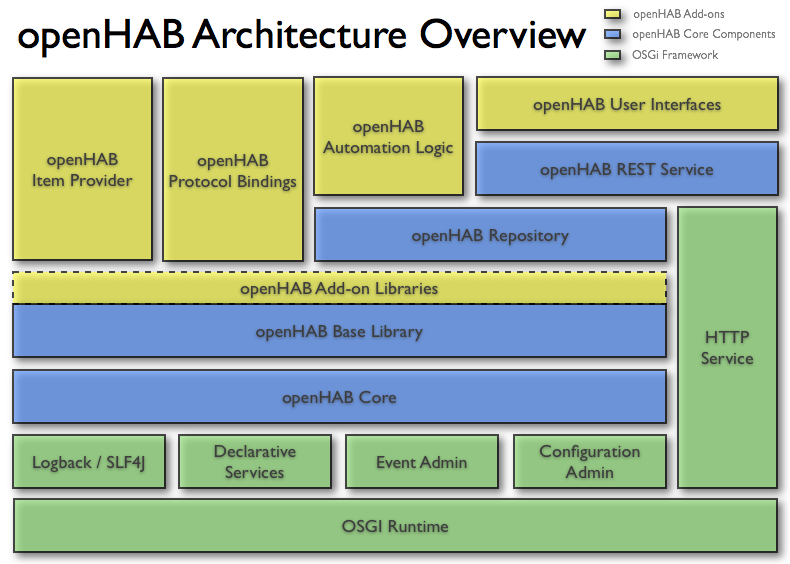
\includegraphics[width=12cm,height=12cm,keepaspectratio]{images/openhab-architecture.png}
        \caption{Architektur der openHAB Plattform \cite{openHAB-architecture2018}}
        \label{fig:architectureopenHAB}
    \end{figure}

    %Describe the concepts 

    %Dinge
    %Dinge sind die Entitäten, die physisch zu einem System hinzugefügt werden können und die potenziell viele Funktionalitäten 
    %in einem bereitstellen können. Es ist wichtig zu beachten, dass Dinge nicht Geräte sein müssen, sondern auch einen 
    %Webdienst oder jede andere überschaubare Informationsquelle und Funktionalität darstellen können. Aus Benutzersicht 
    %sind sie für den Einrichtungs- und Konfigurationsprozess relevant, nicht aber für den Betrieb.
    %Dinge können Konfigurationseigenschaften haben, die optional oder obligatorisch sein können. Solche Eigenschaften können 
    %grundlegende Informationen wie eine IP-Adresse, ein Zugriffstoken für einen Webdienst oder eine gerätespezifische 
    %Konfiguration sein, die sein Verhalten ändert.
    %1) Kanäle: Dinge stellen „Kanäle“ bereit, die die verschiedenen Funktionen darstellen, die das Ding bereitstellt. Wo das 
    %Ding die physische Entität oder Informationsquelle ist, ist der Kanal eine konkrete Funktion von diesem Ding. Eine 
    %physische Glühbirne kann einen Farbtemperaturkanal und einen Farbkanal haben, die beide die Funktionalität der einen 
    %Glühbirne für das System bereitstellen. Als Informationsquellen könnte das lokale Wetter mit Informationen von einem 
    %Webdienst mit verschiedenen Kanälen wie Temperatur, Druck und Luftfeuchtigkeit dienen.
    %Kanäle sind mit Elementen verknüpft, wobei solche Verknüpfungen der Klebstoff zwischen der virtuellen und der physischen 
    %Ebene sind. Sobald eine solche Verbindung hergestellt ist, reagiert ein Ding auf Ereignisse, die für ein Element gesendet 
    %werden, das mit einem seiner Kanäle verknüpft ist. Ebenso sendet es aktiv Ereignisse für Artikel, die mit seinen Kanälen 
    %verknüpft sind.
    %2) Brücken: Eine besondere Art von Ding ist eine „Brücke“. Brücken sind Dinge, die dem System hinzugefügt werden müssen, 
    %um Zugriff auf andere Dinge zu erhalten. Ein typisches Beispiel für eine Bridge ist ein IP-Gateway für ein nicht 
    %IP-basiertes Hausautomationssystem oder eine Webdienstkonfiguration mit Authentifizierungsinformationen, die alles von 
    %diesem Webdienst benötigen könnte.




\subsection{Ziele und Schwerpunkte}
\subsection{Stärken und Schwächen}

\section{Vergleich von Home Assistant und openHAB}
\label{sec:comparison-HAOS-openHAB}
    %Allgemein gültiger Vergleich (Aufbau, Architektur, Schwerpunkte (Fokus), Umsetzungen, Konnektivität, etc.)
    % https://everythingsmarthome.co.uk/home-assistant-vs-openhab-which-one-is-better/
    % https://smarthome.msuttner.de/openhab-2/vergleich-openhab-vs-home-assistant/ 
    % https://www.electronicshub.org/openhab-vs-home-assistant/ 
    % https://smarthome.university/your-smart-home-platform-home-assistant-vs-openhab/ 

